\documentclass{article}[18pt]
\usepackage{../../../../format}
\lhead{Software Methodologies - Machine Learning}


\begin{document}
\begin{center}
\underline{\huge Introduction to Machine Learning}
\end{center}
\section{Machine Learning Lifecycle}
\begin{center}
	\includegraphics[scale=0.7]{"Machine Learning Lifecycle"}
\end{center}
\begin{center}
	\includegraphics[scale=0.7]{"Machine Learning Lifecycle1"}
\end{center}
\begin{itemize}
	\item Randomise the data order so that the model doesn't train for specific orders
	\item Two types of data, training and evaluation, to train and assess the model respectively 
	\item To determine how to differentiate between things using our model rather than using human judgement and manual rules
	\item We can extrapolate the ideas to other problem domains as well, where the same principles apply
\end{itemize}
\section{What is machine learning?}
\begin{defin}[Machine Learning]
A computer program is said to learn from experience E with respect to some class of tasks T and performance measure P if its performance at tasks in T, as measured by P, improves with experience E.
\end{defin}
Machine learning is the study of algorithms that:
\begin{itemize}
	\item Improve their performance P
	\item At some task T
	\item With experience E
\end{itemize}
A well defined learning task is given by \texttt{<P,T,E>}
\section{Supervised Learning (regression)}
To learn the mapping (the rules) between a set of inputs and outputs\\
\\
Labelled data is provided of past input and output pairs during the learning process to train the model how it should behave
\section{Unsupervised learning}
To learn the hidden pattern (the rules) from a set of inputs (no output)\\
\\
Unlabelled data is provided of past input during the learning process to train the model how it should behave\\
\\
\textbf{Dimensionality reduction} - Get rid of unused parameters and aspects of the system
\section{Reinforcement learning}
Occasional positive and negative feedback is used to reinforce behaviours
\begin{itemize}
	\item Good behaviours are rewarded with a treat and become more common
	\item Bad behaviours are punished and become less common
\end{itemize}
A reinforcement learning algorithm just aims to maximise its rewards by playing the game over and over again
\begin{center}
	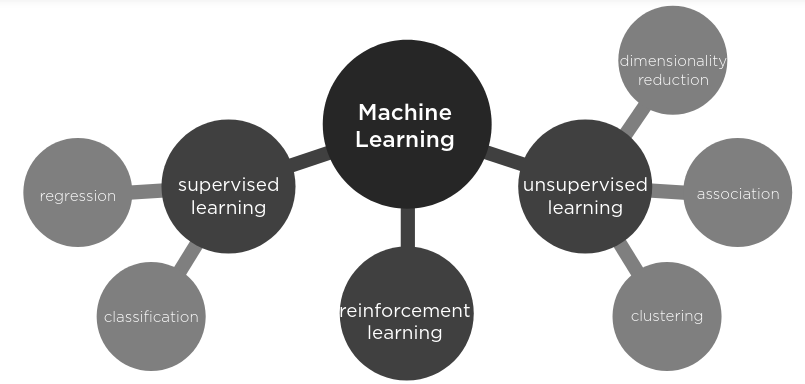
\includegraphics[scale=0.7]{Categories}
\end{center}
\section{Key terms}
\textbf{Label} - The variable that we are predicting typically represented by the variable y\\
\textbf{Features} are input variables that describe our data typically represented by the variables ${x_1,x_2,x_3,...,x_n}$\\
\textbf{Example} - A particular instance of data, x\\
\textbf{Labelled example} - Has \{features,label\}:(x,y) used to train the model\\
\textbf{Unlabelled example} - Has \{feature,?\}:(x,?) used for making prediction on new data\\
\textbf{Model} - Maps examples to predict labels: $\hat{y}$ defined by internal parameters, which ate learned\\
\textbf{Training} - Creating or learning the model\\
\textbf{Inference} - Applying the trained model to unlabelled examples



\end{document}